\chapter{費米子符號與超對稱相消}

\lectureoverview{超對稱將玻色子與費米子聯繫起來，但在寫下其代數之前，先看看為何需要這種關係會更容易理解。我們先從旋轉的拓撲談起，接著透過干涉讓費米子波函數的符號成為可觀測量，再由交換反對稱性推導閉合費米子圈的負號，最後運用玻色子圈與費米子圈符號相反這一點，說明真空能與標量自能為何可能相消。後半部則探討超對稱可以破缺到什麼程度、如何探測超對稱伴粒子，以及為什麼精確超對稱會抹去一般原子的殼層結構。}

\section{超對稱之前：旋轉的一個奇特之處}

超對稱是費米子與玻色子之間的對稱性。然而，在嘗試構造這種對稱性之前，不妨先回想這兩類粒子對旋轉的反應有多麼不同。這個問題始於一個拓撲事實：它很容易演示，但看過之後卻令人難以忘懷。

手掌朝上，轉動手腕\(2\pi\)。手回到原來的朝向，但手臂顯然沒有回到等價的狀態：它扭轉了。再轉\(2\pi\)，必要時讓手臂跟著移動，就能解開扭轉。因此，在周圍環境保持固定時，\(2\pi\)旋轉無法連續形變至無旋轉，而\(4\pi\)旋轉則可以。這個手部演示，字面上說，就是一種「揮手證明」。

不借助人體解剖也能說明同一件事。把一顆球放在固定的盒子裡，用任意多條柔軟、可伸展但不會斷裂的繩子，將球連接到盒壁。讓球旋轉一周，轉過\(2\pi\)。繩子會糾纏起來，單靠移動繩子無法恢復原來的狀態。若球總共轉過\(4\pi\)，就能讓繩子繞著球移動，直到糾纏解開。盒壁代表空間無窮遠；這個比較之所以有意義，是因為邊界沒有跟著球一起旋轉。

\begin{classroomqa}
\audiencequestion{能不能轉動盒子來解開繩子的糾纏？\lecturetimestamp{00:02:53}}
\lecturerresponse{那就改變了問題。盒子代表空間無窮遠，因此保持固定。我們比較的是物體相對於周圍環境的旋轉，而不是物體與環境一起旋轉。}
\end{classroomqa}

\begin{classroomqa}
\audiencequestion{為什麼不把球再轉\(2\pi\)？\lecturetimestamp{00:03:20}}
\lecturerresponse{這正是兩種情形的差別。若不再繼續轉動球，一次\(2\pi\)旋轉留下的糾纏就無法解開。再轉一周，總共轉過\(4\pi\)之後，糾纏便能解開。}
\end{classroomqa}

用現代群論的語言來說，旋轉群的閉合路徑有兩種拓撲類別：
\begin{equation}
\pi_1\!\left(SO(3)\right)\cong \mathbb Z_2.
\end{equation}
遍歷一次屬於非平凡類別，遍歷兩次則屬於平凡類別。
換句話說，\(SU(2)\)是\(SO(3)\)的雙重覆蓋。這便是費米子符號的幾何前史。

\editorialnote{\(SO(3)\)、\(SU(2)\)與基本群等數學語言，讓拓撲結構一目了然。手臂和繩子的演示則從幾何上呈現了同樣的二值性。}

\section{\texorpdfstring{\(2\pi\)}{2 pi}旋轉對量子態的作用}

現在固定粒子的位置，只考慮它的自旋態，記為\(\ket{\psi}\)。整數自旋粒子是玻色子，半整數自旋粒子是費米子。要實現物理旋轉，可以將帶電自旋置於強磁場中並轉動磁場，也可以讓自旋在固定磁場中進動所需的角度。

\begin{classroomqa}
\audiencequestion{在實驗室裡，究竟要如何旋轉電子自旋？\lecturetimestamp{00:05:26}}
\lecturerresponse{磁場提供了操控自旋的方式。可以轉動足夠強的磁場，讓自旋跟著磁場轉動；也可以讓自旋繞著固定磁場進動。徒手抓住電子並不是可行的實驗方法。}
\end{classroomqa}

假設完整旋轉\(2\pi\)會使量子態乘上一個相位：
\begin{equation}
R(2\pi)\ket{\psi}=\xi\ket{\psi}.
\end{equation}
將此操作執行兩次，得到
\begin{equation}
R(4\pi)\ket{\psi}=\xi^2\ket{\psi}.
\end{equation}
由於\(4\pi\)路徑在拓撲上屬於平凡類別，在這裡的比較中，它必須等同於恆等操作。因此
\begin{equation}
\xi^2=1,
\qquad
\xi=+1\ \hbox{or}\ -1.
\end{equation}
玻色子對應正號，費米子對應負號：
\begin{align}
R(2\pi)\ket{\psi_B}&=+\ket{\psi_B},\\
R(2\pi)\ket{\psi_F}&=-\ket{\psi_F}.
\end{align}
對於自旋確定為\(j\)的態，可以簡潔地寫成
\begin{equation}
R(2\pi)=(-1)^{2j}.
\end{equation}
逐字稿簡短地說，第二種可能是乘以\(2\pi\)；但從前後推導及板書論證可知，原意應是乘以\(-1\)。

乍看之下，這似乎沒有物理意義。若整個波函數變號，
\begin{equation}
\Psi\longmapsto-\Psi,
\end{equation}
機率仍然不變，因為
\begin{equation}
(-\Psi)^*(-\Psi)=\Psi^*\Psi.
\end{equation}
準備兩組狀態相同的電子，將其中一組的每個電子旋轉\(2\pi\)，另一組則保持不動。對任何單獨電子進行測量，都無法判斷它來自哪一組。整體相位不是可觀測量。

\section{讓負號成為相對量}

若只對波函數的一個相干分支施加符號變化，而不影響另一分支，這個符號就能被觀測到。讓電子逐一通過雙路徑裝置。不要測定電子走哪條路徑，因為路徑資訊會破壞干涉。令上、下兩條路徑的振幅分別為\(\psi_1\)與\(\psi_2\)，重新合併後的態就是
\begin{equation}
\Psi=\psi_1+\psi_2.
\end{equation}
設想暫時將兩個分支各自限制在一個磁場區域內。只將第二個分支所經區域的磁場旋轉\(2\pi\)。若粒子是費米子，態便變為
\begin{equation}
\Psi'=\psi_1-\psi_2.
\end{equation}
這就不再是整體符號變化。相對相位會使干涉極大值與極小值互換。若返回的兩個波包以探測器中央為對稱中心、互為鏡像，反對稱組合在中央便會相消為零：
\begin{equation}
\Psi'(0)=\psi_1(0)-\psi_2(0)=0.
\end{equation}
因此，在這個對稱點絕不會探測到電子。若改為同時旋轉兩個分支，則會得到\(-\psi_1-\psi_2=-\Psi\)，不會產生可觀測效應。

講座強調這項實驗的關係性。讓一個磁場區域相對於另一個區域旋轉，就像球旋轉而盒子保持固定；讓兩個區域一起旋轉，則像球和盒子一起轉動。相對旋轉\(4\pi\)會使效應消失，因為此時費米子態回到原狀時帶有正號。這項實驗由 Yakir Aharonov 與 Leonard Susskind 於1967年提出，講座也順帶提到，它後來以干涉儀實現。同一原理也適用於電子或帶電離子：若干涉條紋移動，表示自旋為半整數；若條紋不移動，則表示自旋為整數。

\begin{classroomqa}
\audiencequestion{若相對磁場轉過\(4\pi\)，移動後的條紋會回到原來的位置嗎？\lecturetimestamp{00:12:21}}
\lecturerresponse{會。兩次符號變化相乘得到\(+1\)，造成極大值與極小值互換的相對相位便消失了。}
\end{classroomqa}

\begin{classroomqa}
\audiencequestion{盒子裡的繩子應該在多大程度上被視為與費米子有字面上的關聯？\lecturetimestamp{00:13:43}}
\lecturerresponse{那些繩子是用來記憶拓撲的比喻，並非真的繫在電子上的物理繩子。玻色子的行為就像轉過\(2\pi\)後不留任何痕跡；費米子則恰好保留了非平凡糾纏所代表的符號痕跡。}
\end{classroomqa}

\begin{classroomqa}
\audiencequestion{兩個磁場區域裡各有一個電子嗎？一個被旋轉，另一個沒有？\lecturetimestamp{00:14:29}}
\lecturerresponse{不是。只有一個電子，處於相干的空間疊加態。它有振幅分布在兩個分支上，而裝置不能揭露它位於哪個分支。旋轉一個區域會改變一個振幅相對於另一個振幅的相位；同時旋轉兩個區域則只會改變共同相位。}
\end{classroomqa}

角度\(2\pi\)很特殊，因為自旋方向會回到原狀，而旋量會多出一個負號。一般的相對旋轉也會改變自旋方向。若兩條路徑的自旋態分別以\(\ket{\chi_1}\)和\(\ket{\chi_2}\)返回，干涉項便正比於
\begin{equation}
\braket{\chi_1}{\chi_2}.
\end{equation}
其大小決定條紋的可見度。\editorialnote{自旋重疊公式是對講座中干涉部分減弱或完全消失之定性討論的標準補充。}若自旋態彼此正交，就能完整判定粒子走過哪條路徑，因此不會發生干涉。

\begin{classroomqa}
\audiencequestion{如果測量電子位於哪個磁場區域，會發生什麼事？\lecturetimestamp{00:18:03}}
\lecturerresponse{干涉圖樣會消失。任何能分辨兩條路徑的紀錄，都會破壞兩個振幅的相干疊加。}
\end{classroomqa}

\begin{classroomqa}
\audiencequestion{如果所有自旋一開始都朝同一方向，最後再測量自旋，\(2\pi\)這項操作本身會改變那個方向嗎？\lecturetimestamp{00:18:17}}
\lecturerresponse{不會。經過\(2\pi\)旋轉後，物理上的自旋方向仍與原來相同；只有費米子分支多了一個負號。正因如此，這項操作可以改變干涉，卻不會留下不同的自旋方向作為路徑標記。}
\end{classroomqa}

\begin{classroomqa}
\audiencequestion{如果磁場只轉過\(\pi\)，而不是\(2\pi\)，會怎麼樣？\lecturetimestamp{00:18:43}}
\lecturerresponse{那麼自旋方向就會改變。上自旋分支與下自旋分支可以彼此區分，因此無法干涉。中間角度會使可見度逐漸降低；相對旋轉\(180^\circ\)則會使干涉完全消失。}
\end{classroomqa}

\section{交換對稱性與閉合圈的符號}

旋轉的討論已經揭示一個費米子負號。全同粒子交換時，還會出現另一個密切相關的符號。對於雙粒子波函數，
\begin{align}
P_{12}\Psi_B(1,2)&=+\Psi_B(1,2)=+\Psi_B(2,1),\\
P_{12}\Psi_F(1,2)&=-\Psi_F(1,2)=-\Psi_F(2,1).
\end{align}
玻色子態具有對稱性，費米子態則具有反對稱性。

\begin{figure}[htbp]
\centering
\includegraphics[width=0.74\textwidth]{lecture_02_figure_02.png}
\lectureframe{00:24:27}
\caption{以態記號表示的交換論證。畫面中只有 ket 標記能確實辨認；反對稱性方程式是排印於正文中，並未聲稱是被遮擋的板書內容。}
\end{figure}

現在不必計算積分，就能判定閉合粒子圈的相對符號。考慮一個沒有外腿的真空費曼圖。可以把它想成粒子在時空中走過一條閉合路徑，也可以想成一對粒子與反粒子產生後又湮滅。這種真空圖會貢獻於真空振幅，因而也貢獻於真空能。

先考慮兩個互不連通的圈。不連通圖的貢獻相乘；因此，若單一圈的符號為\(\sigma\)，兩個圈的符號便是
\begin{equation}
\sigma^2=+1.
\end{equation}
在同一時刻，例如\(t=0\)，將兩個圈都切開。這個時間切片上有兩個全同粒子。不交換粒子便重新接合，會恢復成兩個分離的圈；若在接合前交換兩個粒子，拓撲便變成單一的圈。交換對玻色子貢獻\(+1\)，對費米子則貢獻\(-1\)。由於起初兩個圈的符號乘積為正，最後單一圈的符號就是
\begin{equation}
\begin{aligned}
\operatorname{sign}(\text{closed boson loop})&=+1,\\
\operatorname{sign}(\text{closed fermion loop})&=-1.
\end{aligned}
\end{equation}
更一般地，含有\(L_F\)個獨立閉合費米子圈的圖，會帶有因子
\begin{equation}
(-1)^{L_F}.
\end{equation}
講座刻意從粒子交換推導這條規則，而不訴諸格拉斯曼積分。這個初等論證清楚呈現了符號的物理起源。

\section{相反的圈符號與真空能}

玻色子真空圈以一種符號增加真空能的貢獻，費米子圈則以相反符號貢獻。這立刻帶來啟發：觀測到的暗能量密度，與量子場論中粗略的截斷估算相比，極其微小。講座引用的這項著名差異約為\(123\)個數量級。確切的指數取決於採用哪個紫外尺度；關鍵在於兩者之間驚人的落差。

圈圖的貢獻不只取決於統計性質，也取決於質量、電荷、多重度與交互作用。然而，若玻色子與費米子在所有相關性質上都相匹配，它們大小相同的貢獻便可能相消：
\begin{equation}
\begin{gathered}
m_B=m_F,\qquad q_B=q_F,\qquad g_B=g_F,\\
\Delta\rho_{\mathrm{vac}}^{(B)}
+\Delta\rho_{\mathrm{vac}}^{(F)}=0.
\end{gathered}
\end{equation}
這個觀察並未解決宇宙學常數問題，只是提供了普通玻色子圈無法提供的東西：符號相反的貢獻。在適當假設下，精確未破缺的全域超對稱理論確實能使真空能精確相消；超對稱破缺後，觀測到的微小非零值仍未獲得解釋。\editorialnote{這項限定說明，講座提出的動機與更棘手的宇宙學常數問題並非一回事。}

已知精確匹配並不符合自然界的情況。假如電子有一個質量和電荷都相同、自旋為零的伴粒子，電子與正電子經由虛光子湮滅時，就能產生一對這種粒子：
\begin{equation}
e^-e^+\longrightarrow\gamma^*
\longrightarrow\widetilde e^-\widetilde e^+.
\end{equation}
帶電標量粒子若與電子質量簡併，就不可能逃過一般的對撞機實驗。因此，玻色子與費米子之間的對應不可能是觀測到的粒子譜所具有的精確對稱性。這是粒子種類之間的對應，不是物理空間中的反射。

\section{更直接的目標：標量自能}

真空能是第一個例子，但講座主要關注的是標量質量的輻射不穩定性。裸質量為零的標量粒子仍可能受到對截斷尺度呈二次敏感的修正。概略而言，
\begin{equation}
\Delta m_H^2\sim \frac{g_B^2}{16\pi^2}\Lambda^2
\end{equation}
這項修正來自玻色子圈。費米子質量受到另一種機制保護：若無質量費米子具有精確的手徵對稱性，輻射修正就不能產生加法質量項。這就是前一講提到的左右手論證。

現在設想一種足夠嚴格的對稱性，能將標量與費米子納入同一多重態，並使兩者的交互作用相匹配。如此一來，費米子圈就會帶有相反的符號：
\begin{equation}
\Delta m_H^2
\sim
\frac{g_B^2-g_F^2}{16\pi^2}\Lambda^2+\cdots .
\end{equation}
若超對稱要求\(g_B=g_F\)且兩者質量相等，二次項便會相消。如此一來，費米子所受到的保護便延伸到了它的玻色子伴粒子。這不只是兩個費曼圖之間的數值巧合；對稱性必須在每一階及所有允許的交互作用中，確保這種相消。

這幅橫跨整塊黑板的比較，呈現了講座如何從個別圈圖轉向傳播粒子的成對圈圖修正。

\begin{figure}[htbp]
\centering
\includegraphics[width=0.79\textwidth]{lecture_02_figure_04.png}
\lectureframe{00:40:23}

\medskip
\begin{tikzpicture}[scale=0.9]
\draw (-4.2,0) circle (0.55);
\draw[dashed] (-2.4,0) circle (0.55);
\draw (0,0) -- (3.7,0);
\fill (1.85,0) circle (0.055);
\draw (1.85,0) -- (1.85,0.25);
\draw[dashed] (1.85,0.85) circle (0.6);
\end{tikzpicture}
\caption{一般粒子圈圖與伴粒子圈圖拓撲結構的整板對照。排印的草圖只保留了畫面中看得見的拓撲差異，沒有標註被遮擋的粒子名稱。}
\end{figure}

課間休息後，講座從所謂的零階圖像重新開始。這不是微擾論中的階數，而是指最粗略但仍有用的描述：
\begin{quote}
每種粒子都有一個統計性質相反的超對稱伴粒子。每個費米子都有一個玻色子伴粒子，每個玻色子也都有一個費米子伴粒子。
\end{quote}
在精確超對稱理論中，伴粒子也會與原粒子質量簡併，也就是兩者質量相等。自然界並非如此。不過，即使質量不完全相等，只要差距不太大，相消仍可能足以避免標量修正暴增。在軟超對稱破缺下，危險的尺度概略上會由超對稱伴粒子的質量劈裂取代：
\begin{equation}
\Delta m_H^2\sim
\frac{g^2}{16\pi^2}\,\Delta m_{\mathrm{SUSY}}^2
\ln\!\frac{\Lambda^2}{\Delta m_{\mathrm{SUSY}}^2}
\end{equation}
其中還有依模型而異的係數。\editorialnote{這個公式表達了講座中的定性說法：質量無法完全匹配時，會留下由質量劈裂控制的殘餘修正。這個公式並非抄自板書。}

\section{超對稱破缺與2010年的實驗賭注}

這場講座於2010年錄製，當時還沒有觀測到任何超對稱伴粒子。直接的推論是：如果這些伴粒子確實存在，它們必定比已知粒子重，也超出先前實驗設備的探測能力。超對稱模型也區分了兩種粒子：一種只有在電弱對稱性破缺後才取得質量；另一種則可具有較大的、在對稱性保持時就存在的質量。講座以此說明，為什麼超對稱粒子譜中可見的那一半可能較輕，未見的那一半則較重；同時也坦承，這樣的安排有些牽強。Susskind 表示自己預期能探測到超對稱伴粒子，但隨即說明，這只是猜測，並非結論。

因此，大型強子對撞機是這場講座展望的核心。當時預期它會搜尋希格斯玻色子與超對稱伴粒子。這些說法必須放在2010年的背景下理解：講座是在希格斯玻色子發現、以及後來的 LHC 搜尋結果出爐之前，說明當時的實驗賭注。

為什麼受自然性考量驅動的超對稱伴粒子不應該落在普朗克尺度？因為那樣就無法完成它被賦予的任務。若玻色子與費米子的質量相差極大，兩者的圈圖積分在較輕粒子的質量以上便不再相消。剩餘的標量修正大致由較重粒子之間的質量劈裂決定，而非由弱尺度決定。即使超對稱存在於任意遙遠的尺度，它仍是數學上的對稱性，但已無法令人信服地解釋希格斯部門為何如此輕。

講座根據當時的預期，推論相關質量劈裂應在數百 GeV 左右，因此落在 LHC 的探測範圍內。這個數值估計具有時代背景，也取決於模型；更重要的是以下推理：
\begin{equation}
\begin{gathered}
\text{Higgs protection}\\
\Downarrow\\
\text{effective boson--fermion cancellation}\\
\Downarrow\\
\Delta m_{\mathrm{SUSY}}\ \text{not too large}.
\end{gathered}
\end{equation}

\begin{classroomqa}
\audiencequestion{所有費米子貢獻能不能只在總體上抵消所有玻色子貢獻，而不必有一對一對應的伴粒子？\lecturetimestamp{00:45:01}}
\lecturerresponse{數值上確實可能相消，但那會是偶然的相消，其精細調節程度與原本的問題一樣。超對稱的主張更強：合理的假設能確保各項貢獻相匹配，而超對稱破缺則解釋了為什麼質量只能近似匹配。這裡以真空能作為例子；眼前真正關注的是希格斯自能。}
\end{classroomqa}

\begin{classroomqa}
\audiencequestion{若說總體相消不自然，是否已經預設了以還原論方式組織理論？\lecturetimestamp{00:47:51}}
\lecturerresponse{這是合理的質疑。沒有人對自然性有最終定義，而尋找解釋本身也多少是在摸索，試圖找到一種令人信服的說法。超對稱與自發超對稱破缺提供了已知的數學架構，能確保所需的相消模式。尚待解答的是：自然界是否採用這套架構？它是否獨一無二？}
\end{classroomqa}

\section{直接產生、虛粒子效應與衰變鏈}

重粒子即使未以殼上態產生，也可能影響實驗。它可以作為虛粒子出現在圈圖內部，稍微改變一般電子與正電子的散射振幅。因此，即使質心能量低於直接產生粒子對的閾值，精密電弱測量仍能限制超對稱伴粒子的性質。
\begin{equation}
\sqrt{s}<2m_{\widetilde p}.
\end{equation}
講座在2010年的評估是，精密資料已開始壓縮超對稱參數空間，但還沒有將超對稱排除。

\begin{classroomqa}
\audiencequestion{能不能像早先對某些重粒子的情況一樣，在直接觀測之前，根據精確的產生率間接推斷超對稱伴粒子？\lecturetimestamp{00:49:01}}
\lecturerresponse{可以。虛超對稱伴粒子圈圖會稍微改變一般的散射振幅，因此問題就轉為高精度電弱現象學，而不是直接產生。若有一座環境乾淨、能量足夠高的電子正子對撞機，會特別有幫助。質子碰撞則比較複雜，因為質子是由夸克和膠子組成的複合態；實際碰撞的是不斷漲落的組成粒子，而不是初始條件明確已知的兩個基本粒子。}
\end{classroomqa}

一名學生問，能否反過來進行這種反應，從大量超粒子開始。問題不在時間反演對稱性，而在於能否取得這些粒子。必須先產生重的超對稱伴粒子，而其中大多數預期會迅速衰變為較輕的態。

\begin{classroomqa}
\audiencequestion{如果某個宇宙中有很多超粒子，兩個超粒子能不能碰撞並轉變成一般粒子？\lecturetimestamp{00:53:43}}
\lecturerresponse{原則上，相關反應存在逆向通道，但重的超對稱伴粒子不太可能以自由粒子的形式大量存在。它們會衰變至較低能量的態，因此實驗必須先提供足夠的碰撞能量，才能產生這些粒子。}
\end{classroomqa}

這就帶出了暗物質的問題。在許多超對稱模型中，一條離散選擇定則會阻止衰變鏈末端的超對稱伴粒子完全消失。因此，每個較重的超對稱伴粒子都會級聯衰變，最後到達最輕超對稱伴粒子（LSP）。若 LSP 是電中性的，它就可能穩定且難以探測，因此可作為暗物質候選者。逐字稿在這段對話中有一次說成「暗能量」，但聽眾的提問和對粒子的描述都明確指向暗物質。

\begin{classroomqa}
\audiencequestion{超對稱伴粒子快速衰變，會不會與某種超對稱伴粒子可能構成暗物質的說法互相矛盾？\lecturetimestamp{00:54:53}}
\lecturerresponse{不會。在要求每條衰變鏈末端都留下一個超對稱伴粒子的模型中，大多數伴粒子可以衰變，最輕的那個則保持穩定。帶電粒子通常會帶來額外的現象學難題，因此可行的 LSP 很可能是電中性的。它並非原理上不可探測，但不會像帶電超電子那樣留下明顯的電離軌跡。}
\end{classroomqa}

\section{匹配也包括耦合常數}

只匹配質量還不夠。比較電子真空圈與超電子圈：兩者的統計性質不同，因而符號相反；要使貢獻大小相等，還需要質量相等。再接上兩個外部光子。係數也含有電磁耦合，因此相消還要求電荷相等：
\begin{equation}
\begin{gathered}
q_{\widetilde e}=q_e,\\
\mathcal A_{\mathrm{loop}}^{(e)}
+\mathcal A_{\mathrm{loop}}^{(\widetilde e)}=0,\\
\text{provided the full couplings match.}
\end{gathered}
\end{equation}
任何一處不匹配，都會留下未相消的發散項。超對稱的價值在於，它不只關聯粒子的名稱與自旋，也關聯它們的交互作用。

\begin{figure}[H]
\centering
\includegraphics[width=0.66\textwidth]{lecture_02_figure_05.png}
\lectureframe{00:57:15}

\medskip
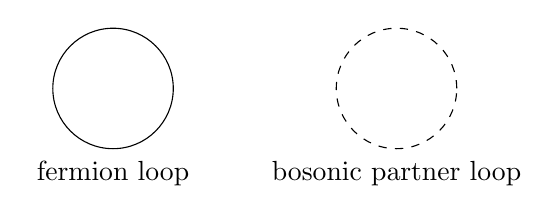
\begin{tikzpicture}[scale=0.9]
\draw (-2.0,0) circle (0.85);
\draw[dashed] (2.0,0) circle (0.85);
\node at (-2.0,-1.2) {fermion loop};
\node at (2.0,-1.2) {bosonic partner loop};
\end{tikzpicture}
\caption{電荷匹配論證中用來比較的實線圈圖與虛線圈圖。由於僅憑畫面無法判定每個外部端點如何連接，因此沒有補畫遭裁切的外部標記。}
\end{figure}

\begin{classroomqa}
\audiencequestion{超對稱伴粒子會不會只是因為耦合常數不同，才一直沒有被探測到？\lecturetimestamp{00:56:23}}
\lecturerresponse{若要求相同的費曼圖彼此相消，就不會是這樣。加入光子交互作用後，就能檢驗每條粒線所帶的電荷。耦合不相等會使圈圖因子大小不同，於是大幅殘餘項又會出現。對稱性必須確保相應的電荷與交互作用相匹配。}
\end{classroomqa}

\begin{classroomqa}
\audiencequestion{光子的超對稱伴粒子也應該是無質量的嗎？\lecturetimestamp{00:58:01}}
\lecturerresponse{在精確超對稱理論中，它會是無質量的，因為它與光子質量簡併。觀測到的世界並非精確超對稱，因此實際存在的類光微子態不必與光子質量相同。}
\end{classroomqa}

\section{超對稱伴粒子名稱一覽}

這些命名規則不算優雅，但很實用。玻色子的費米子伴粒子名稱通常以\emph{-ino}結尾，例如光子與光微子、\(W\)與 wino、\(Z\)與 zino、膠子與膠微子、希格斯玻色子與希格斯微子、引力子與引力微子。一般費米子的玻色子伴粒子名稱，通常以\emph{s-}開頭，例如電子與超電子、夸克與超夸克。

\begin{center}
\begin{tabular}{@{}>{\raggedright\arraybackslash}p{0.40\linewidth}>{\raggedright\arraybackslash}p{0.52\linewidth}@{}}
\toprule
普通態 & 超對稱伴子與自旋變化\\
\midrule
標量希格斯場，\(j=0\) & 希格斯微子，\(j=\tfrac12\)；\(\Delta j=+\tfrac12\)\\
規範玻色子，\(j=1\) & 規範微子，\(j=\tfrac12\)；\(\Delta j=-\tfrac12\)\\
物質費米子，\(j=\tfrac12\) & 超費米子，\(j=0\)；\(\Delta j=-\tfrac12\)\\
引力子，\(j=2\) & 引力微子，\(j=\tfrac32\)；\(\Delta j=-\tfrac12\)\\
\bottomrule
\end{tabular}
\end{center}

一般而言，同一超多重態中的成員自旋相差半個單位：
\begin{equation}
\Delta j=\frac12.
\end{equation}
講課中舉的粗略例子，是將自旋為\(\tfrac12\)的物質費米子與標量配成一對，以及將自旋為一的規範玻色子與自旋為\(\tfrac12\)的規範微子配成一對。完整的相互作用模型在對稱性破缺後可能發生態混合，因此物理質量本徵態未必沿用這些最簡單的名稱。

\begin{classroomqa}
\audiencequestion{所有新的標量伴子都可能各自發生自發對稱性破缺嗎？\lecturetimestamp{01:01:27}}
\lecturerresponse{標量場可以取得真空期望值，但任意的額外對稱性破缺在現象學上會造成災難性的後果。可行的超對稱模型必須妥善安排標量勢，避免色對稱、電荷對稱及其他必要的對稱性以不適當的方式破缺。}
\end{classroomqa}

\begin{classroomqa}
\audiencequestion{希格斯微子是否有與希格斯四次項相對應的特殊相互作用？\lecturetimestamp{01:02:19}}
\lecturerresponse{超對稱不只使粒子彼此配對，也使相互作用彼此配對。這種關係並非把每條希格斯線直接換成希格斯微子線就能得到；標量四次項，以及相關的費米子與輔助場相互作用，都屬於同一個受約束的結構。講課尚未進一步說明這些細節。}
\end{classroomqa}

\begin{classroomqa}
\audiencequestion{\(2\pi\)旋轉與\(4\pi\)旋轉定理在其他維度也有類似的結果嗎？\lecturetimestamp{01:03:07}}
\lecturerresponse{有，但維度不同，可能的情形也不同。在二維空間中，交換路徑可以彼此纏繞，因此可能出現任意子；它們的交換相位比玻色子的\(+1\)與費米子的\(-1\)更為一般。這類激發會出現在凝聚態系統中，但不在本課程的討論脈絡內。}
\end{classroomqa}

\section{為什麼精確超對稱會抹去化學}

最後，我們來問：一個超對稱完全精確的世界會是什麼樣子？這裡所說的精確，意指每一對粒子與超對稱伴子的質量相等、相互作用相匹配。電子會有一個質量與電荷都相同的玻色子伴子超電子，而無質量的光子則會有一個無質量的費米子伴子光微子：
\begin{equation}
m_{\widetilde e}=m_e,
\qquad
q_{\widetilde e}=q_e,
\qquad
m_{\widetilde\gamma}=m_\gamma=0.
\end{equation}

我們熟悉的化學週期結構仰賴費米統計。氫原子的最低軌域中有一個電子。氦原子在該軌域中容納兩個電子，因為它們的自旋標記不同。鋰的第三個電子必須佔據較高的軌域：泡利不相容原理禁止三個全同電子佔據同一個單粒子態。這個外層電子能量較高，會傾向往內躍遷，通常並伴隨光子放射；但較低能態已被填滿，因此這個躍遷受到阻擋。

精確超對稱開啟了另一種途徑：
\begin{equation}
e^-_{\mathrm{outer}}
\longrightarrow
\widetilde e^-_{\mathrm{inner}}
+
\widetilde\gamma .
\end{equation}
起初的電子與放出的光微子都是費米子，而剩下的超電子是玻色子。超電子遵從玻色統計，而非費米統計，因此即使低軌域中已有粒子，最後的超電子也不會被排除在外。於是，價電子可以轉變成超電子並往內躍遷。

\begin{figure}[H]
\centering
\includegraphics[width=0.62\textwidth]{lecture_02_figure_06.png}
\lectureframe{01:09:18}

\medskip
\begin{tikzpicture}[scale=0.9]
\fill (0,0) circle (0.075);
\draw (0,0) circle (0.72);
\draw (0,0) circle (1.45);
\draw[-{Latex[length=2.2mm]}] (1.42,0.2) .. controls (1.2,0.52) and (0.92,0.42) .. (0.72,0.1);
\draw[decorate,decoration={snake,amplitude=1.4pt,segment length=7pt},-{Latex[length=2.2mm]}]
  (1.58,0) -- (3.55,0);
\node[above] at (2.7,0.12) {$\widetilde\gamma$};
\node[below] at (0,-1.65) {selectron drops to a lower orbital};
\end{tikzpicture}
\caption{這個原子躍遷用來說明精確超對稱為何會改變化學。圖中可見向外射出的波浪線；根據逐字稿，這條線代表光微子。}
\end{figure}

這個結論不只適用於類鋰原子。在大型原子中，化學的多樣性正是由價電子造就的。如果價電子能反覆轉變成玻色子超電子，它們便可能聚集到能量允許的最低區域，而不再填滿各個電子殼層。結果會像是玻色子集中在原子核附近，而非形成我們熟悉的價軌域結構。由方向性鍵與未填滿殼層構成的分子，也將不復存在。講課中把假想的鋰的後代稱為\emph{超鋰}；這個玩笑帶出一個嚴肅的結論：精確超對稱會產生不同於一般化學的物質，因而也不會有一般的生物學。

\begin{classroomqa}
\audiencequestion{電子轉變成超電子的耦合會不會弱到足以讓一般原子存留下來？\lecturetimestamp{01:10:23}}
\lecturerresponse{在我們設想的精確理論中，不會。超對稱將這種轉變與電磁相互作用聯繫起來，因此其耦合強度由電荷決定，不能任意調小。講課中估計類鋰原子的壽命約在微秒量級；這並非精確計算，而是為了強調衰變會很快。}
\end{classroomqa}

因此，光憑日常物質，我們就知道超對稱在低能下不可能是精確的，無須仰賴對撞機搜尋。粒子與其超對稱伴子的質量差，相較於原子或質子的尺度極大；但若與大統一尺度或普朗克尺度相比，這個差距仍可能很小。

\begin{classroomqa}
\audiencequestion{那麼，超對稱為什麼會破缺？\lecturetimestamp{01:11:19}}
\lecturerresponse{講課中提出一個最低限度的選擇性解釋：若超對稱沒有破缺，由一般化學構成的觀測者便不會存在，也就無從提出這個問題。這並不能取代超對稱破缺的動力學理論，只說明了為何低能世界若超對稱完全精確，就不可能是我們所處的世界。}
\end{classroomqa}

超對稱在數學上可以破缺，而且在許多構造中相當普遍；然而，要安排出符合現實的破缺並非自然而然就能做到。另一方面，精確超對稱量子場論具有足夠特殊的結構，使其中某些理論能比一般理論受到更深入的分析。它們既是整理粒子物理學的候選架構，也是格外強大的數學實驗室。下一講將從這項物理動機轉向探討更多這類結構。

\section{論證脈絡}

通往超對稱的論證刻意採取迂迴的路徑：
\begin{enumerate}
\item 空間中的\(2\pi\)旋轉屬於非平凡的拓撲類，而\(4\pi\)旋轉則可以連續變形至恆等變換。
\item 費米子態在\(2\pi\)旋轉下會取得負號；雙路徑實驗顯示，當這個負號是相對的而非全域的時，就能觀測到它。
\item 費米子在交換下的反對稱性，使每個閉合費米子迴圈相較於玻色子迴圈多出一個負號。
\item 當質量與耦合相匹配時，迴圈符號相反便能使對稱性強制真空貢獻與標量自能貢獻彼此抵消。
\item 自然界中並不存在精確的匹配。若超對稱能保護希格斯部門，其破缺就不能讓相關伴子的質量變得任意大。
\item 若低能下的超對稱精確成立，電子便可以轉變成玻色子超電子，使一般化學所依賴的殼層結構崩解。
\end{enumerate}

因此，超對稱之所以引人注目，又不可能以樸素的精確形式存在，原因相同：它將玻色子與費米子緊密地聯繫在一起。這種緊密關係可以抑制危險的量子修正；但如果超對稱不經破缺地延續到原子物理的尺度，這個世界就不會再像我們身處的世界。